\appendix

\begin{frame}{Acknowledgements}
\begin{itemize}
\item My thesis advisor, Professor Chambers
\item Professor Smith for serving as a reader for my thesis
\item Professor Erving for his support as the Honors Program Director
\item Seattle Pacific University for hosting the Northwest Honors Research Symposium
\end{itemize}
\begin{columns}[T,onlytextwidth]
\column{\textwidth}
\begin{minipage}[]{0.15\textwidth}
~
\end{minipage}%
\begin{minipage}[]{0.3\textwidth}
    \begin{centering}
    
\includegraphics[width = \textwidth]{img/SPUTorch_208_LR}
    \end{centering}
\end{minipage}%
\begin{minipage}[]{0.1\textwidth}
~
\end{minipage}%
\begin{minipage}[]{0.3\textwidth}
	\begin{centering}
    
\includegraphics[width = \textwidth]{img/UofPS_stacked_maroonRGB_PNG}
    \end{centering}
\end{minipage}%
\begin{minipage}[]{0.15\textwidth}
~
\end{minipage}%
\end{columns}
\end{frame}

\begin{frame}[standout]
  Questions?
\end{frame}

\begin{frame}[allowframebreaks]{References}

  \bibliography{Mendeley}
  \setbeamertemplate{bibliography item}{\insertbiblabel}
  %\nocite{*} % Insert publications even if they are not cited in the poster
  \bibliographystyle{apalike}
\end{frame}

\begin{frame}{Bio AI}
\begin{figure}
  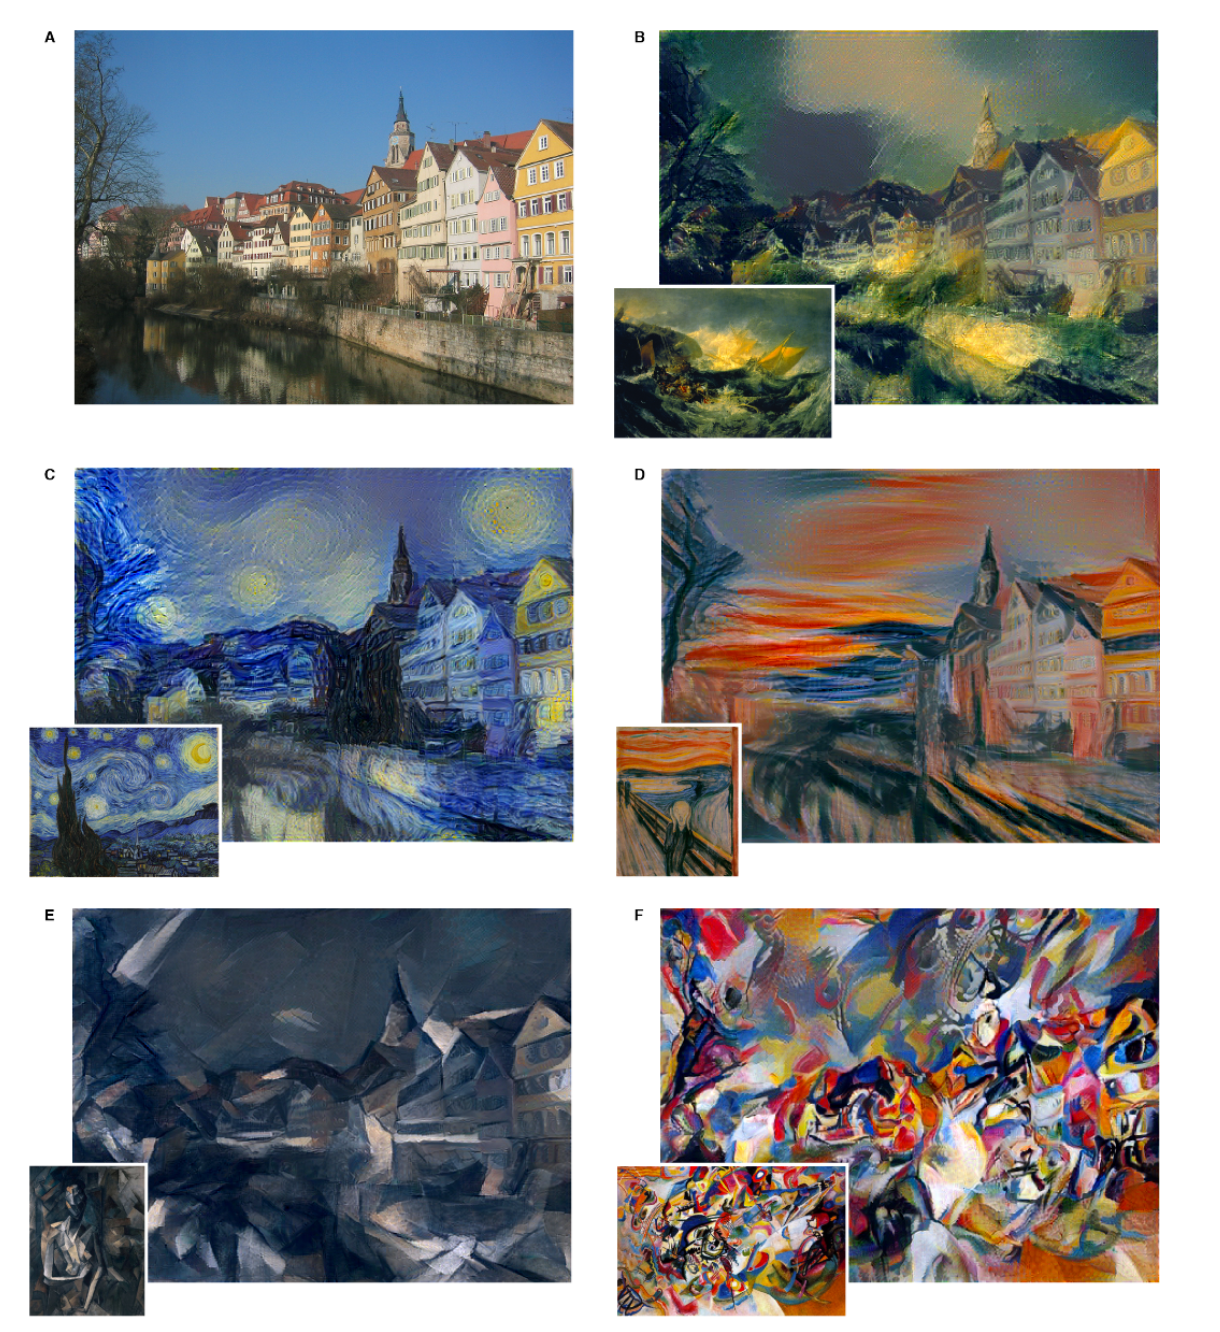
\includegraphics[width=0.6\textwidth]{img/nn_art_styles.png}
  \captionsetup{singlelinecheck=off,justification=raggedright}
  \caption{A Neural Algorithm of Artistic Style \cite{Gatys2015AStyle}}
\end{figure}
\end{frame}

\begin{frame}{Evolvability as Heritable Variation}
  \begin{figure}
 \centering
    \begin{subfigure}[b]{0.5\textwidth}
        \centering
    	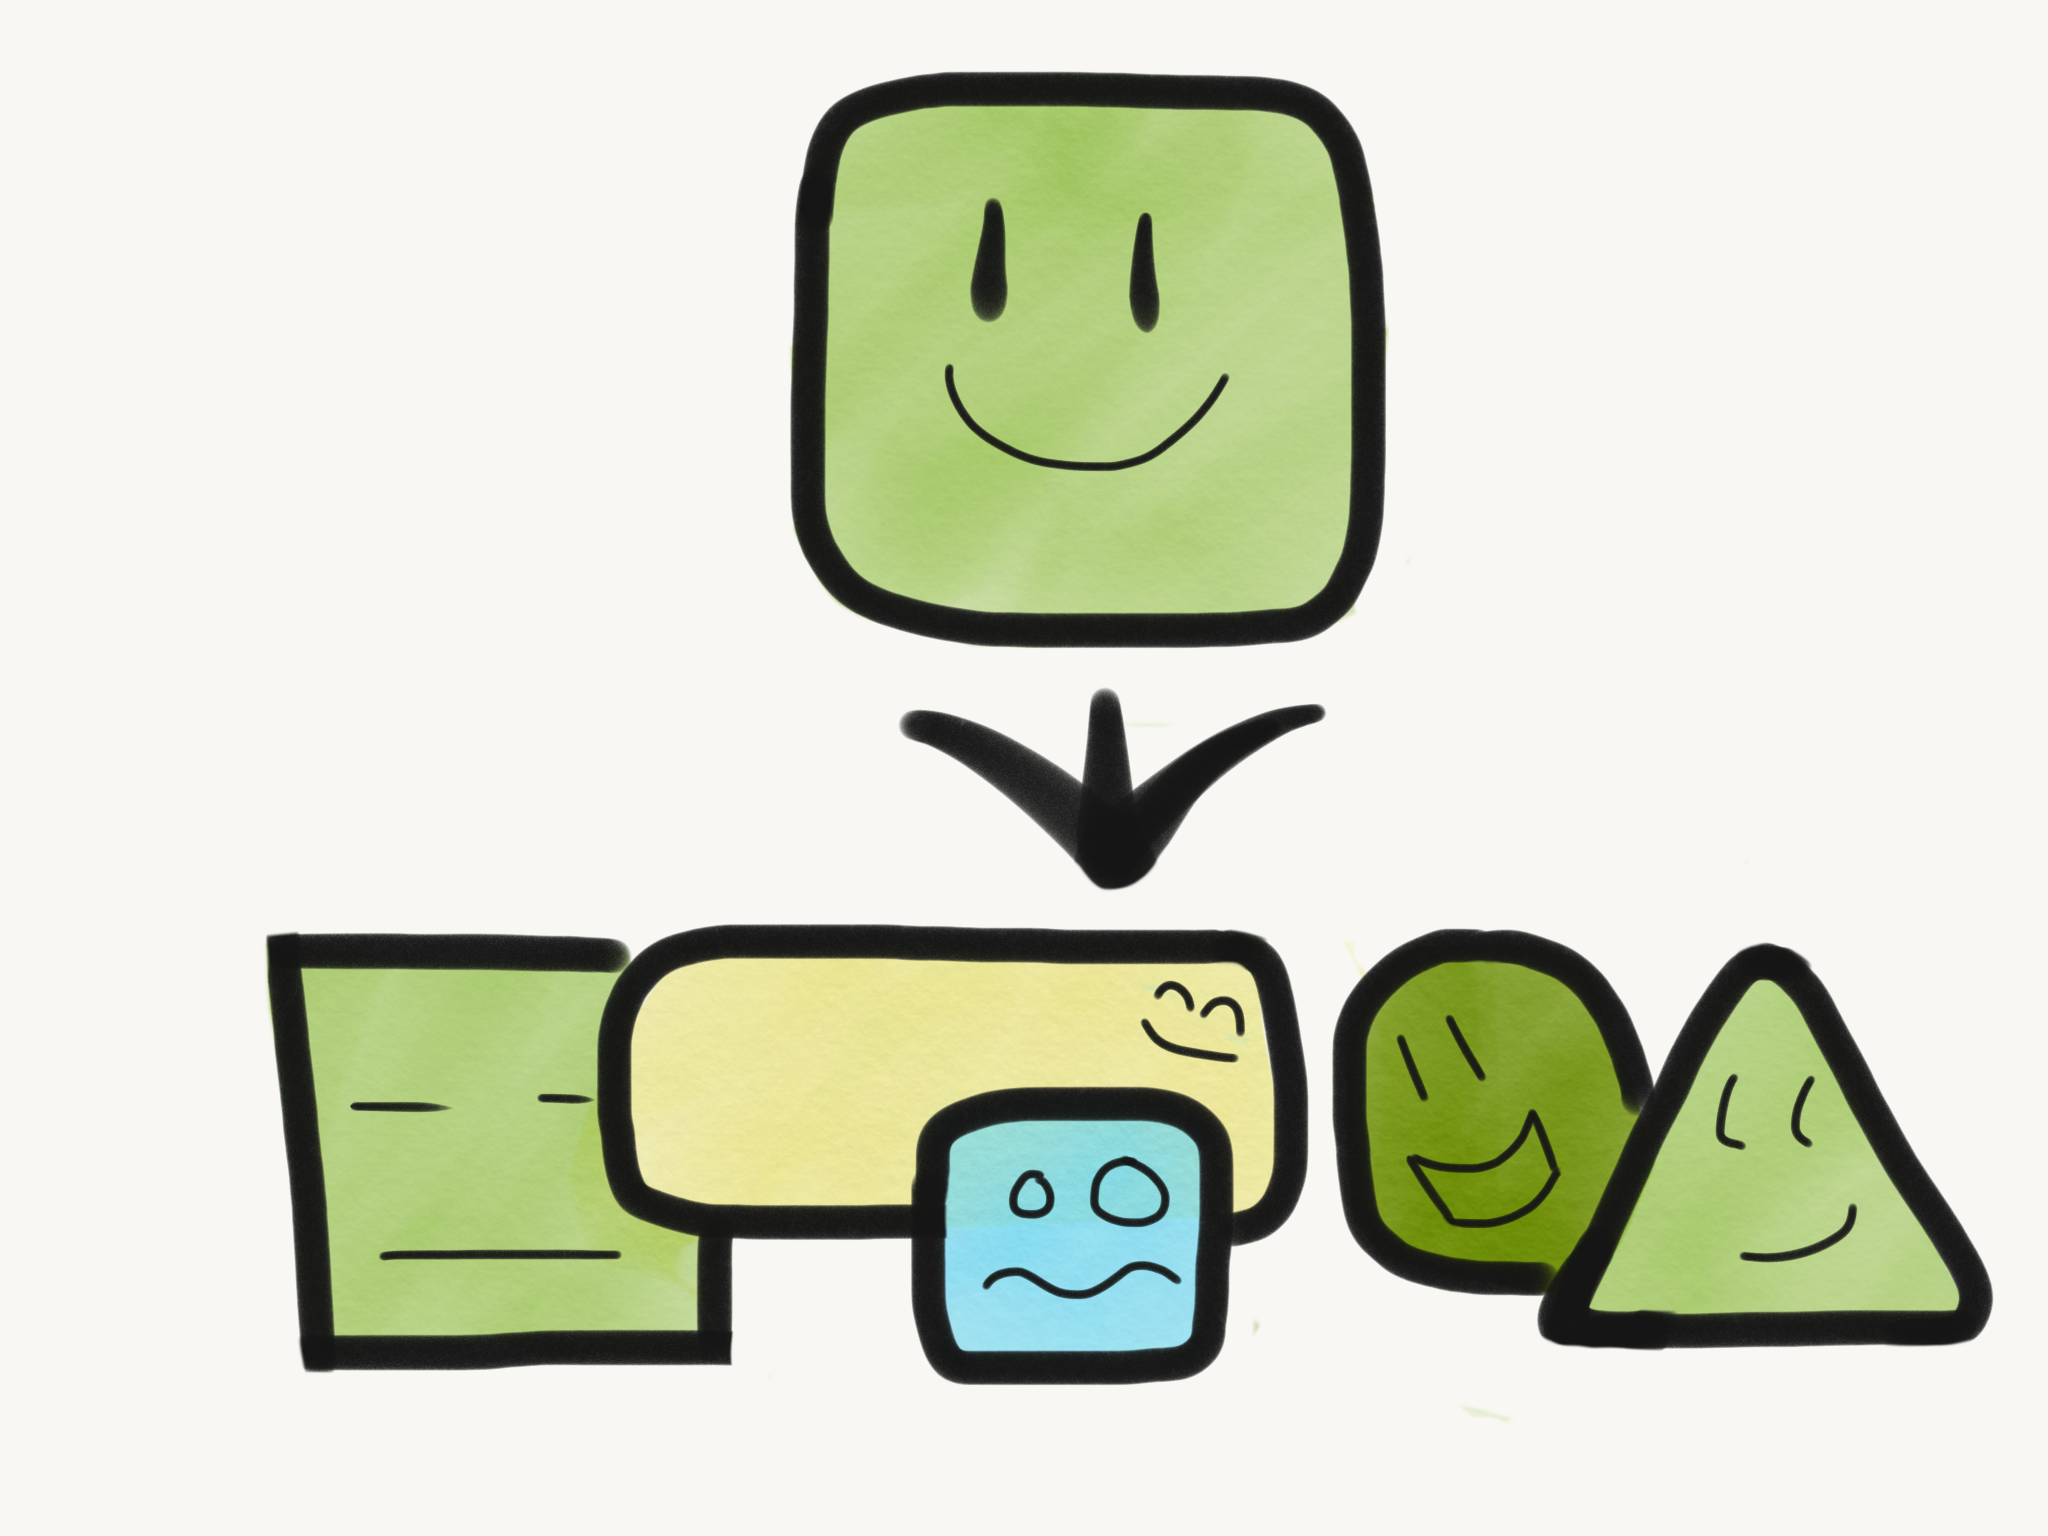
\includegraphics[width=\textwidth]{img/individual_evolvability}
        \caption{individual evolvability}
        \label{subfig:individual_evolvability}
    \end{subfigure}%
    \hfill
    \begin{subfigure}[b]{0.5\textwidth}
        \centering
        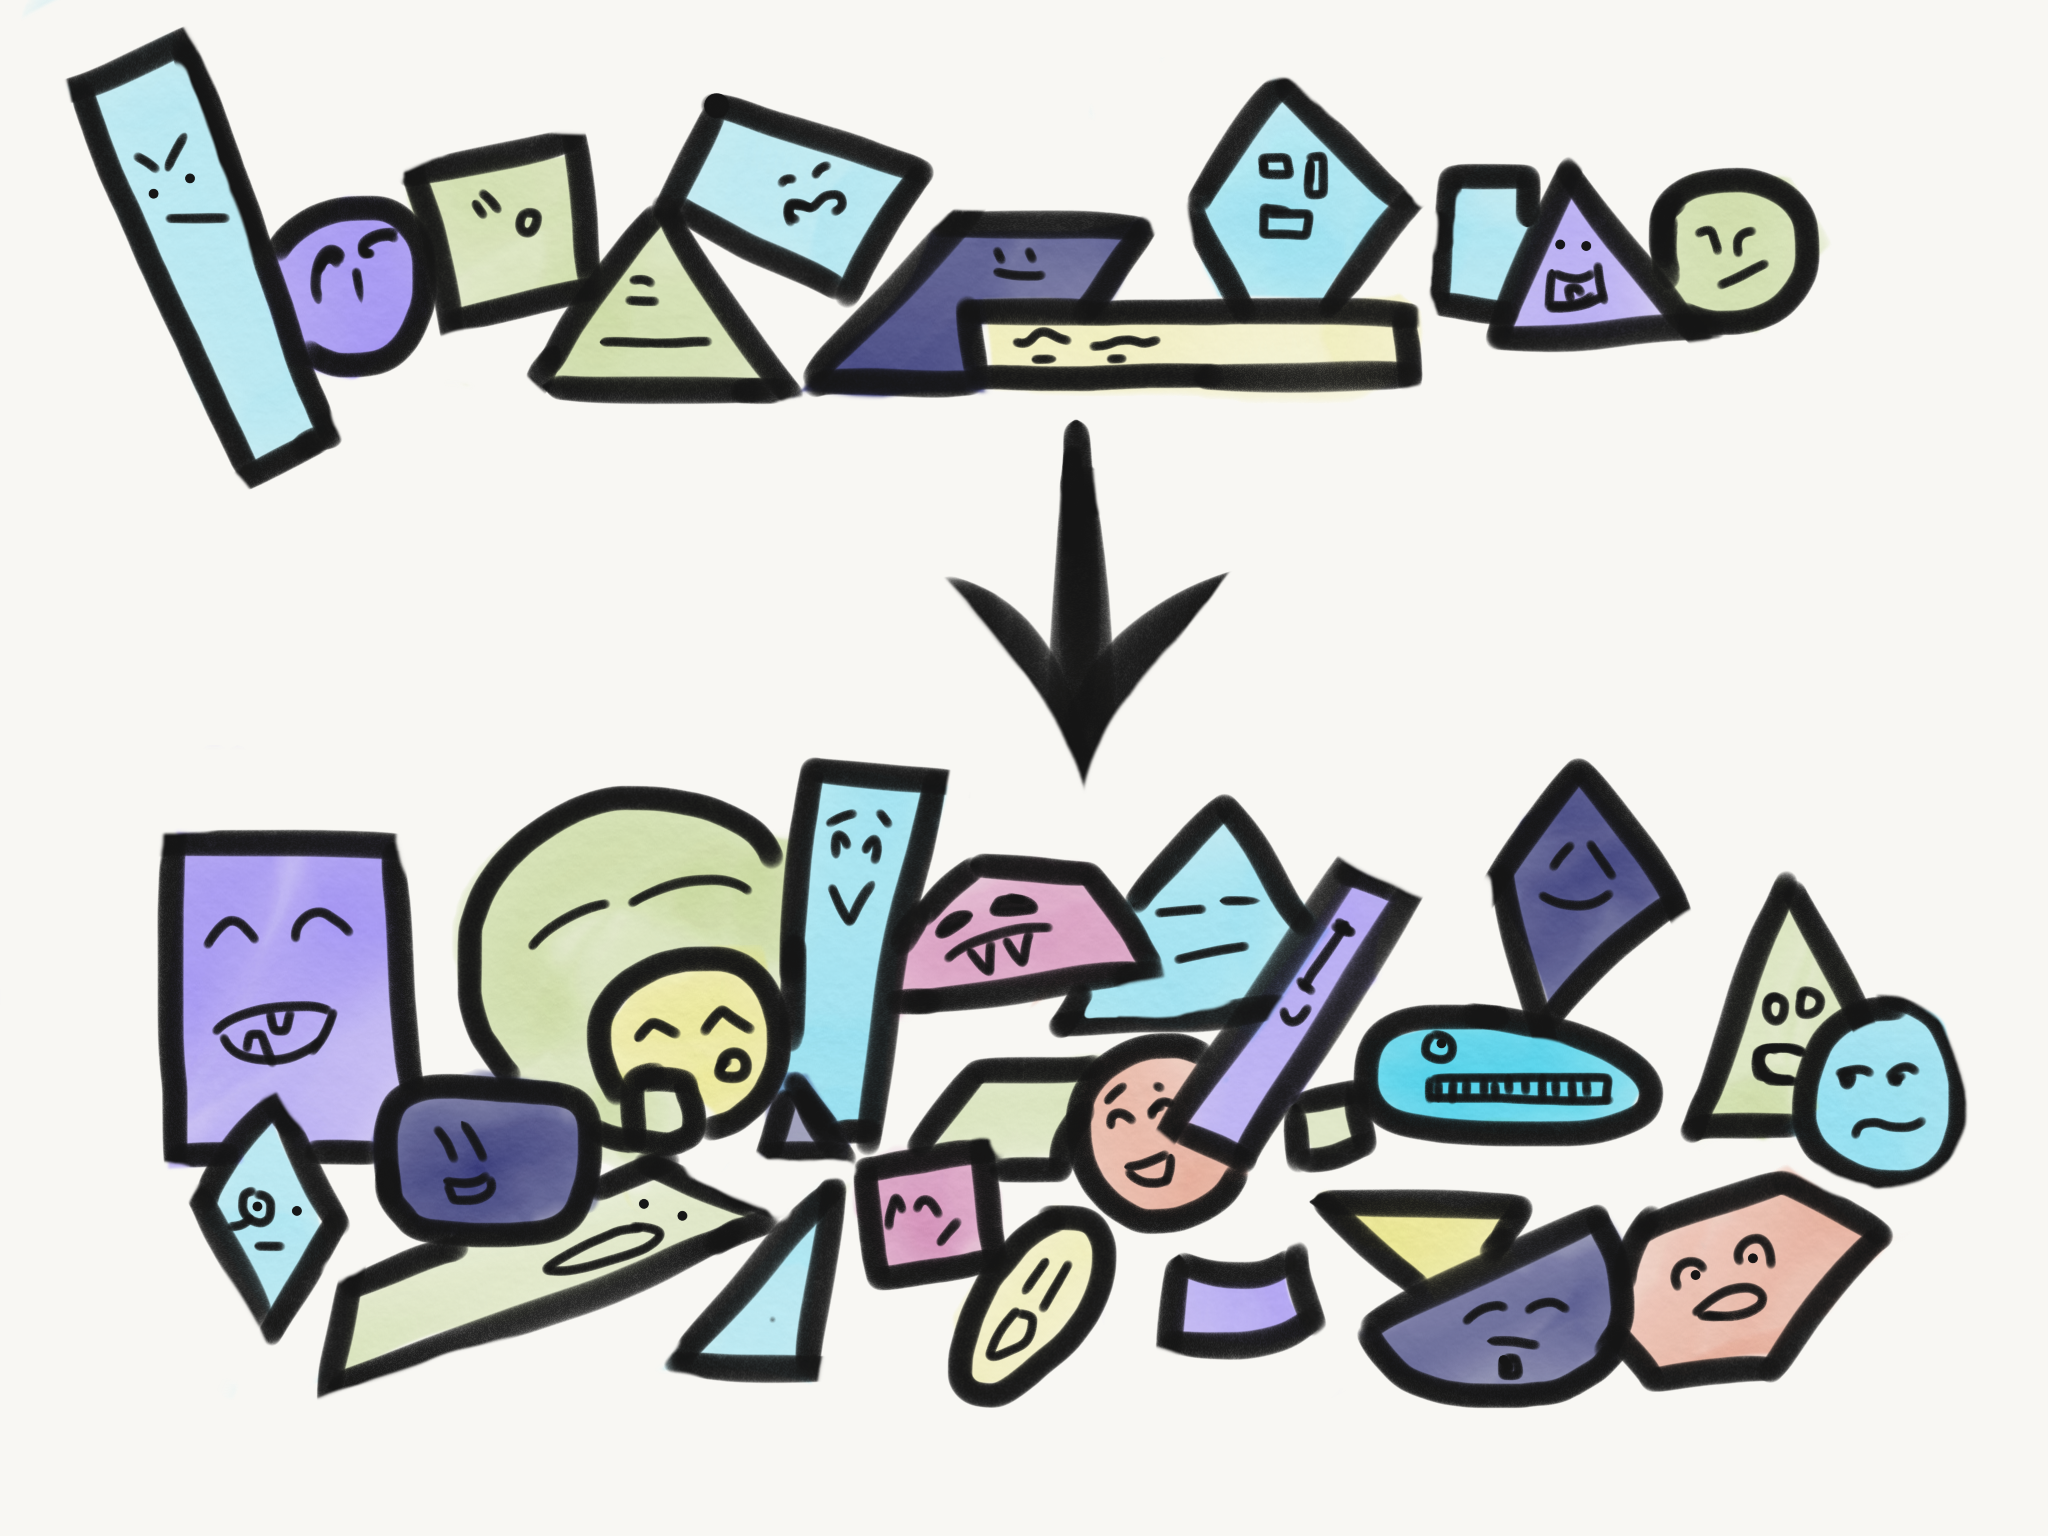
\includegraphics[width=\textwidth]{img/population_evolvability}
        \caption{population evolvability}
        \label{subfig:population_evolvability}
    \end{subfigure}
 	\captionsetup{singlelinecheck=off,justification=raggedright}
    \vspace{-4ex}
  \captionsetup{singlelinecheck=off,justification=raggedright}
  \caption{An illustration contrasting individual and population evolvability \cite{Wilder2015ReconcilingEvolvability}.}
  \label{fig:individual_vs_population_evolvability}
\end{figure}
\end{frame}

\begin{frame}{Evolvability as Bias towards Useful Variation}
  \begin{figure}
    \centering
    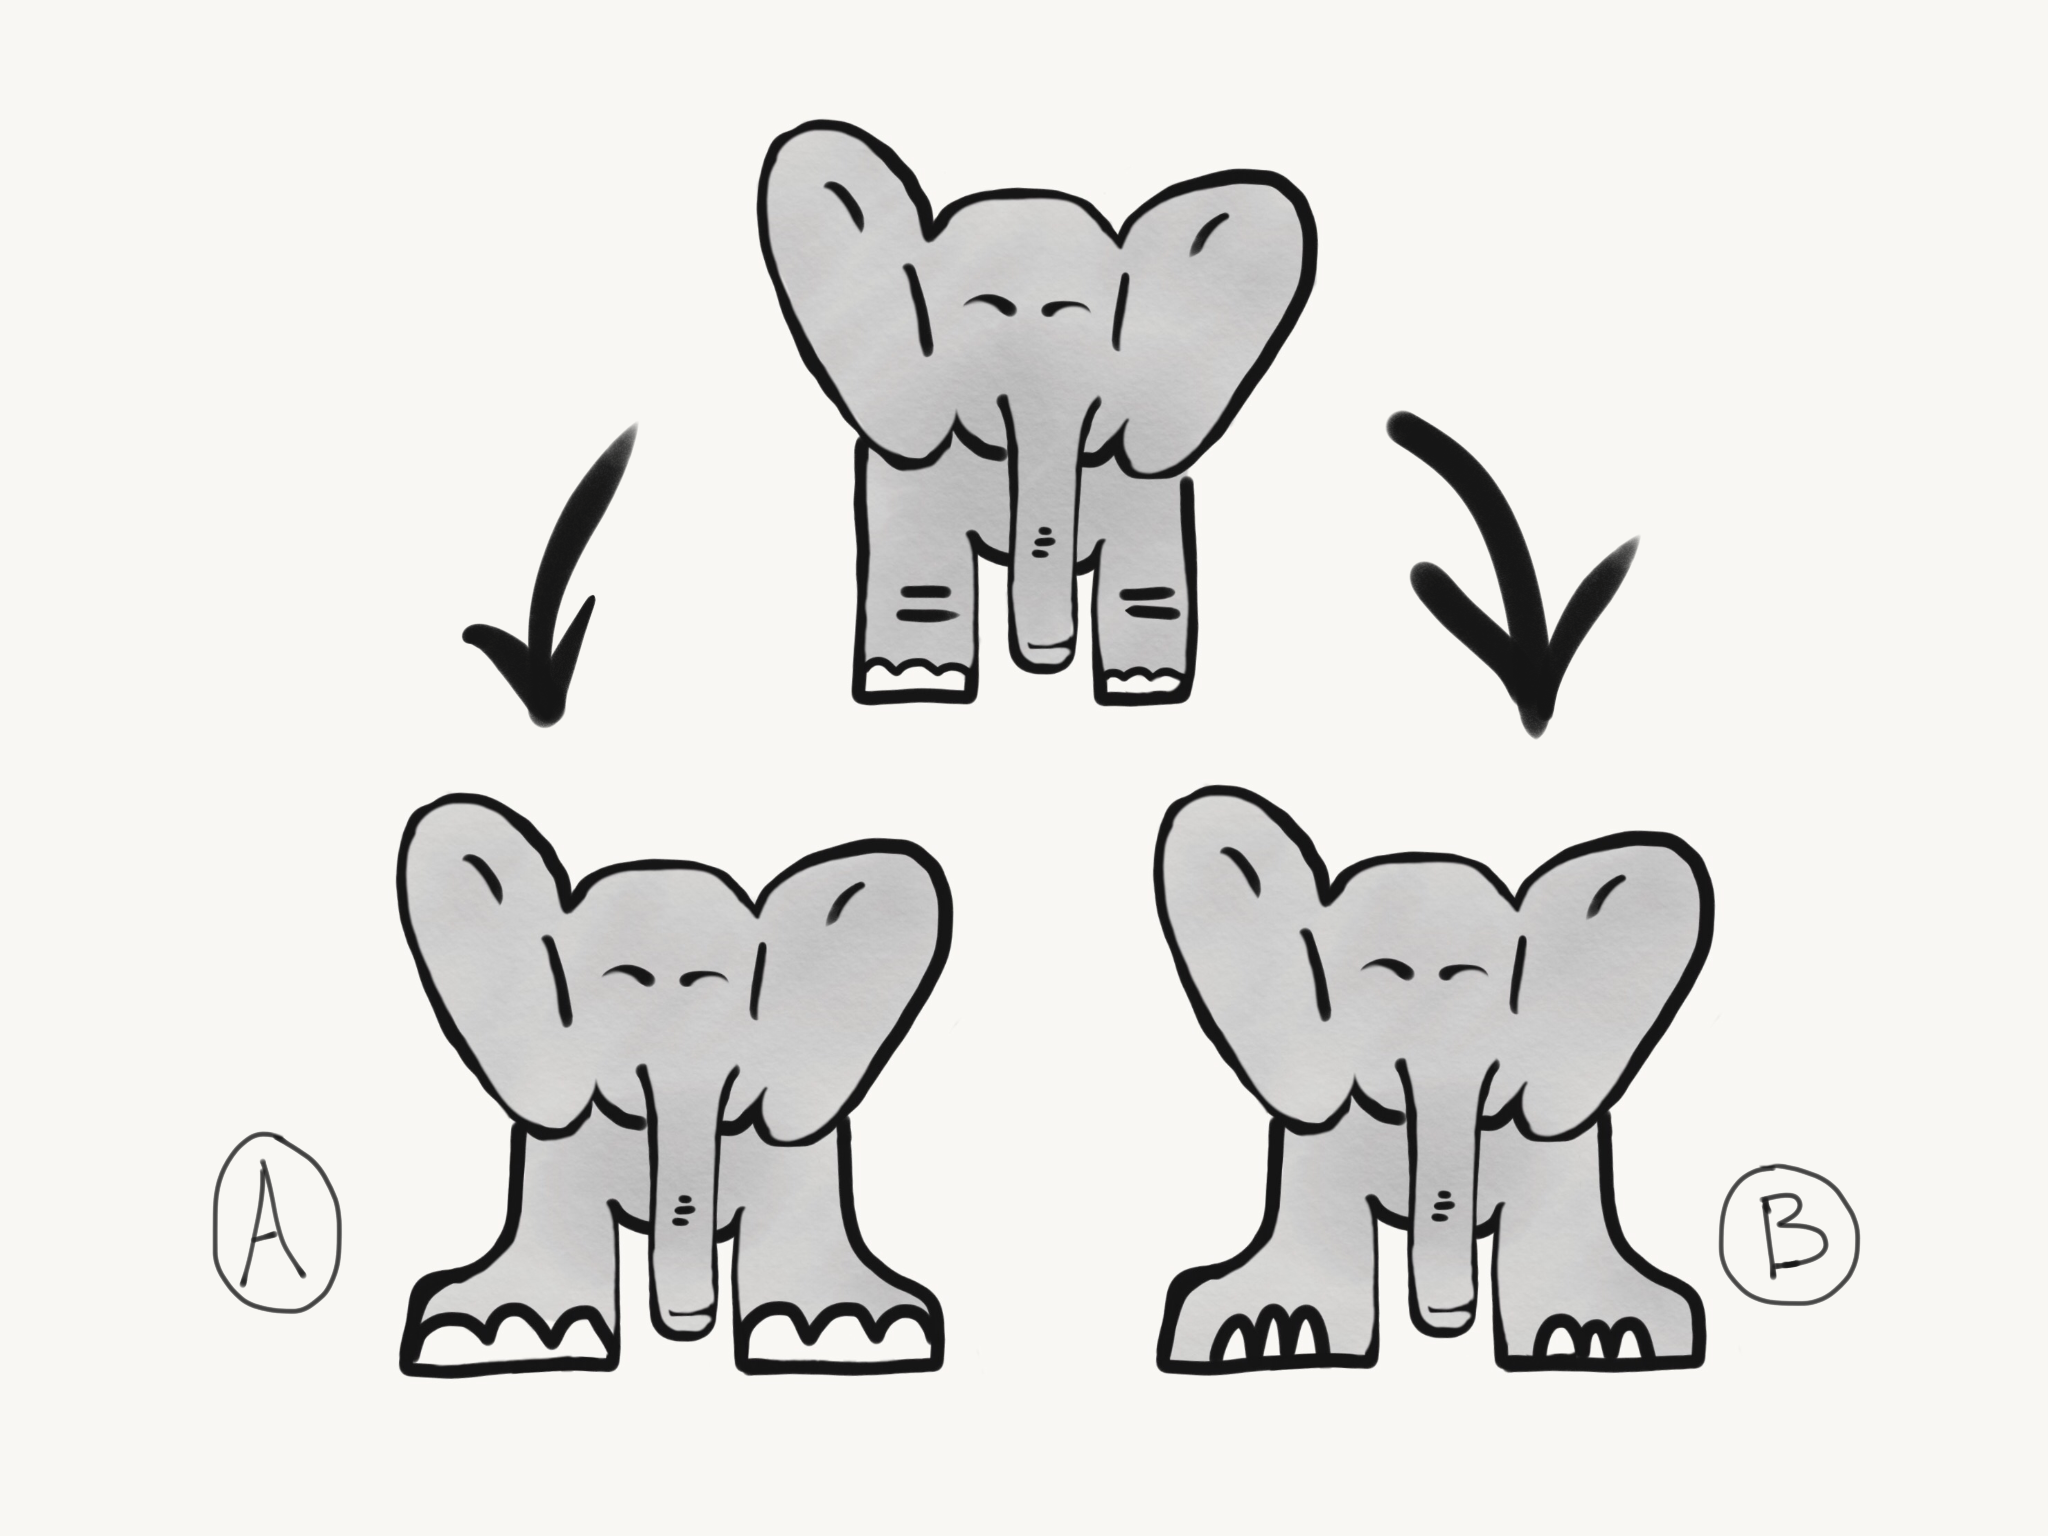
\includegraphics[width=0.8\textwidth]{img/exploratory_growth}
 	\captionsetup{singlelinecheck=off,justification=raggedright}
  	\caption{Illustration of exploratory growth; high evolvability left and low evolvability right \cite{Downing2015IntelligenceSystems}.}
    \label{fig:exploratory_growth}
\end{figure}
\end{frame}

\begin{frame}{Evolvability as Bias towards Useful Variation}
  \begin{figure}
    \centering
    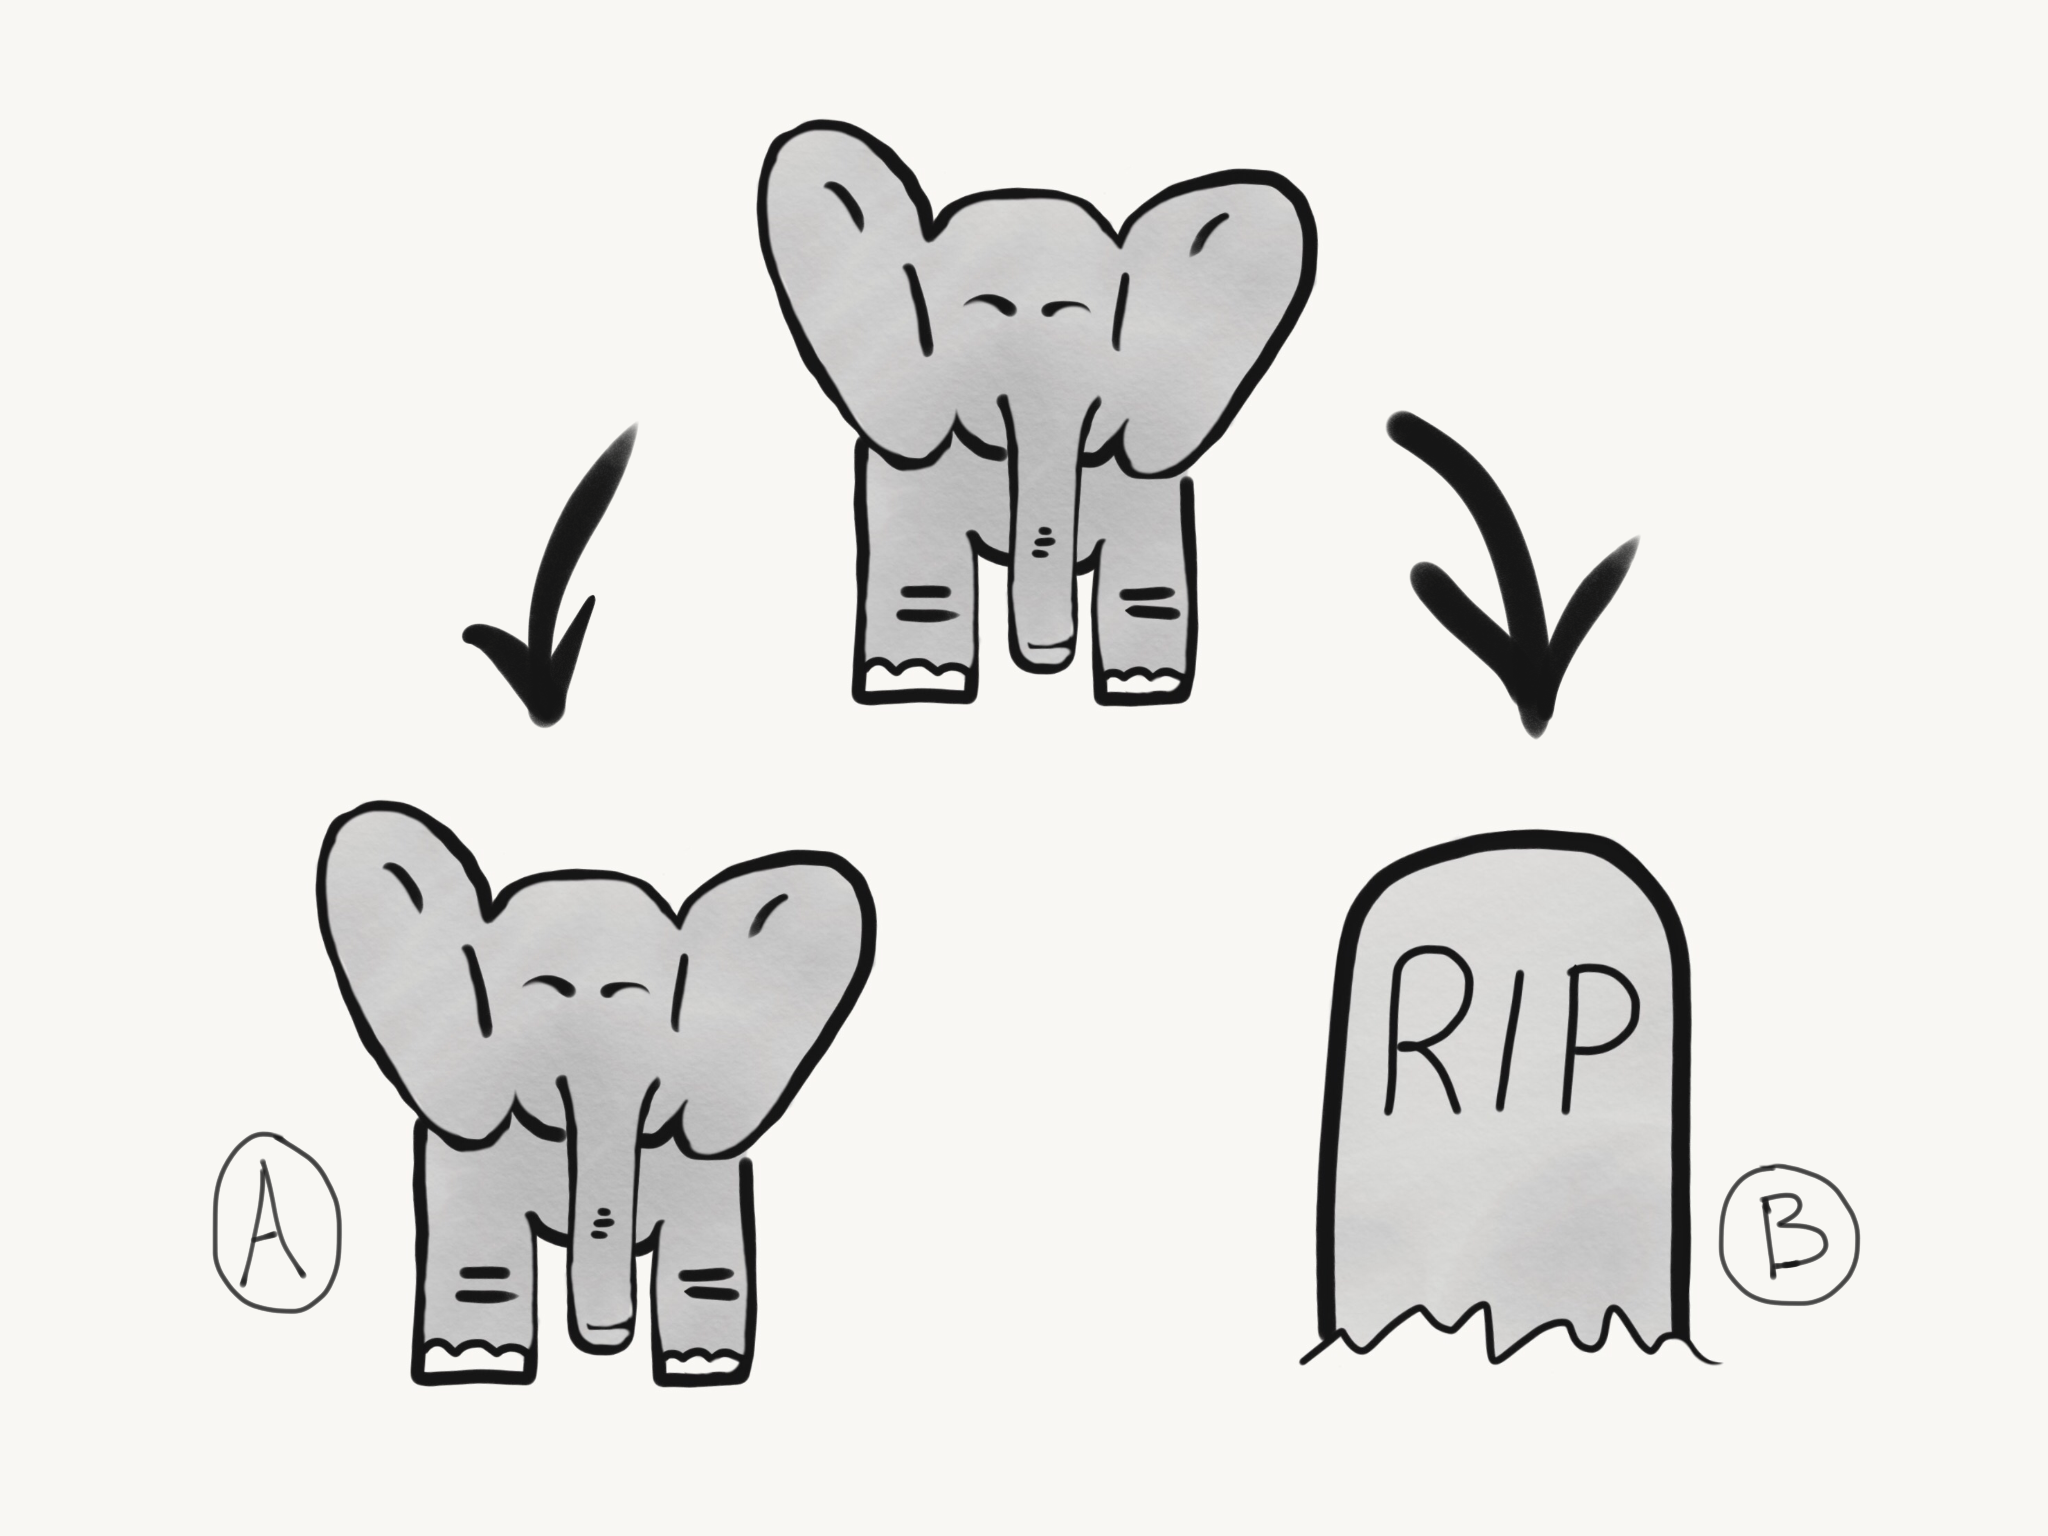
\includegraphics[width=0.8\textwidth]{img/robustness}
 	\captionsetup{singlelinecheck=off,justification=raggedright}
  	\caption{Illustration of robustness; high evolvability left and low evolvability right \cite{Downing2015IntelligenceSystems}.}
    \label{fig:robustness}
\end{figure}
\end{frame}

\begin{frame}{Selection Pressure}
\begin{figure}
\resizebox{\textwidth}{!}{%
	\pgfmathsetseed{1}
\begin{tikzpicture} [x={(-0.2cm,-0.4cm)}, y={(1cm,0cm)}, z={(0cm,1cm)}, scale=1]   

   \begin{scope}[canvas is yx plane at z=0]
     \draw [black!100] (0,2) grid (7,9);
     \draw [black!100] (8,0) grid (19,11);
     
     % primary phenotype mapping
     \foreach \x in {2,3,4}
       \foreach \y in {4,5,6}
    	  \filldraw[fill=pink!40!white, draw=pink] (\x, \y) rectangle (\x+1,\y+1);

     \filldraw[fill=orange!40!white, draw=orange] (3, 5) rectangle (4,6);
     \filldraw[fill=orange!40!white, draw=orange] (13, 5) rectangle (14,6);

      
     \foreach \cx/\cy/\dx/\dy in {2.5/4.5/12.5/8.5,3.5/4.5/15.5/9.5,4.5/4.5/14.5/3.5,2.5/5.5/17.5/5.5,4.5/5.5/11.5/1.5,2.5/6.5/12.5/5.5,2.5/6.5/12.5/5.5,3.5/6.5/12.5/5.5,4.5/6.5/14.5/8.5}
      	\filldraw[fill=pink!40!white, draw=pink] (\dx-0.5, \dy-0.5) rectangle (\dx+0.5,\dy+0.5);
        
      \foreach \x in {8,9,...,18}
       \foreach \y in {0,1,...,10}
        \pgfmathparse{0.9*rnd+0.3}
        \definecolor{MyColor}{rgb}{\pgfmathresult,\pgfmathresult,\pgfmathresult}
        \fill[fill=MyColor, opacity = 0.3] (\x,\y) rectangle (\x+1,\y+1);

      \foreach \cx/\cy/\dx/\dy in {2.5/4.5/12.5/8.5,3.5/4.5/15.5/9.5,4.5/4.5/14.5/3.5,2.5/5.5/17.5/5.5,4.5/5.5/11.5/1.5,2.5/6.5/12.5/5.5,2.5/6.5/12.5/5.5,3.5/6.5/12.5/5.5,4.5/6.5/14.5/8.5}
     	\draw [pink!80!black, line width=2pt] (\cx, \cy) to[bend right=90, in looseness=0.1] (\dx, \dy);

       \draw [orange!80!black, line width=2pt] (3.5,5.5) to[bend right=90, in looseness=0.1] (13.5,5.5);
     
     \draw [black] (3.5,10)node {\LARGE Genotype Space};
     \draw [black] (13.5,12)node {\LARGE Phenotype Space};

   \end{scope}
 \end{tikzpicture}
}
\captionsetup{singlelinecheck=off,justification=raggedright}
\caption{average performance of local genetic environment \cite{Reisinger2005TowardsEvolvability}}
\end{figure}
\end{frame}

\begin{frame}{Bio AI}
\begin{figure}
  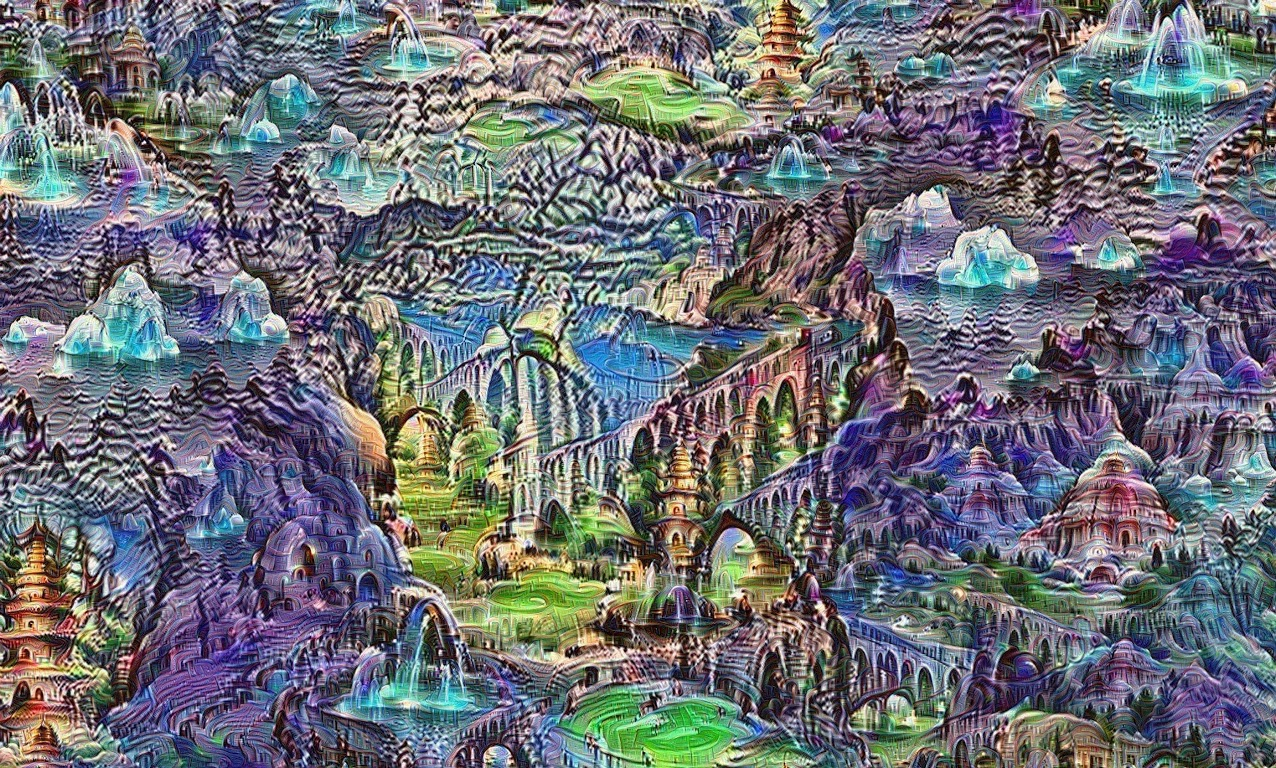
\includegraphics[width=\textwidth]{img/iterative_places}
\captionsetup{singlelinecheck=off,justification=raggedright}
\caption{Google Deep Dream \cite{Mordvintsev2015Inceptionism:Networks}}
\end{figure}
\end{frame}

% \begin{frame}{Measuring Evolvability}
% \begin{itemize}
%   \item amount of information able to acquire (different speeds of varying fitness function)\cite{Reisinger2005TowardsEvolvability} 
%   \item RMS distance in behavioral characterization space (population diversity), ``We approximate an individual’s capacity to generate
% future phenotypic variation by measuring phenotypic
% variability among a sample of the individual’s simulated off-
% spring (which are discarded). Such variability is quantified as
% the number of unique behaviors; in particular, each offspring
% is considered sequentially and added to a list of unique behaviors
% only if its behavior is significantly different from the
% behaviors of organisms already in the list. Two behaviors are
% considered different if the distance between them according
% to a domain-specific behavioral distance metric is above a
% pre-specified threshold'' \cite{Mengistu2016EvolvabilityIt}
%   \item ``a measurement of evolvability should characterize the
% amount of variability that can be accessed in an individual or population's genetic neighborhood; number of distinct phenotypes in a genetic neighborhood around individual; amounts to Monte Carlo sampling of the phenotypic space surrounding an individual \cite{Wilder2015ReconcilingEvolvability}
%   %\item \cite{Tarapore2015EvolvabilityBenchmarks}
% \end{itemize}
% \end{frame}